\stcmt{main points that I want to provide background about them in this section - main focuses: motivating the need for Go correctness, dynamic tracing, bug detection and exposure acceleration, coverage models}

\begin{itemize}
  \item explain concurrency primitives and identify their roles in nondeterministic behaviour of Go concurrency model using the example in listing \ref{listing:moby28462}.
  \item Dynamic tracing - gain insight into the dynamic behavior - detect bugs
  \item injecting random delays
  \item defining coverage metrics to measure the quality of tests
\end{itemize}

\stcmtside{whole subsection is copied from F-IDE, OK to skip review}
\subsection{Go Concurrency}
%
%\stcmtside{Go concurrency introduction}
Go introduces a new concurrency model, mixing shared-memory and message-passing concepts with an ad-hoc scheduler:
\begin{itemize}
    \item \textbf{Goroutines} are functions that execute concurrently on logical processors having their own stack.
    \item \textbf{Channels} are typed conduits through which goroutines communicate.  Channels are unbuffered by default, providing synchronous (rendezvous) messaging between goroutines.
    \item \textbf{Synchronization} features such as \textit{mutex}, \textit{waitGroup}, \textit{conditional variables}, \textit{select}, and \textit{context} are included in the language to provide more and flexible synchronization, data access serialization, memory protection, and error handling.
    \item \textbf{Scheduler} maintains goroutines in FIFO queues and binds them on OS threads to execute on processing cores.
\end{itemize}

\ignore{Due to the unpredictable interaction between components and inherent nondeterminism introduced by the scheduler, concurrent programming and debugging has traditionally been challenging.
%
}

%\begin{listing}[]
\centering
\begin{minted}
[
fontsize=\scriptsize,
linenos=true,
escapeinside=||,
breaklines
]
{go}
package main
import "sync"

type Container struct{ |\label{bugListing:containerType_start}|
  sync.Mutex
  stop  chan struct{}
} |\label{bugListing:containerType_end}|

func main() {
  container := &Container{ |\label{bugListing:container_create_start}|
       stop:make(chan struct{})} |\label{bugListing:container_create_end}|
  go Monitor(container) |\label{bugListing:main_go_monitor}|
  go StatusChange(container) |\label{bugListing:main_go_statChange}|
}
%|\setcounter{FancyVerbLine}{15}|func Monitor(cnt *Container){
func Monitor(cnt *Container){
  for{
    select{
    case <- cnt.stop:  |\label{bugListing:Monitor_case_recv}|
      return |\label{bugListing:Monitor_case_recv_ret}|
    default: |\label{bugListing:Monitor_case_def}|
      cnt.Lock()  |\label{bugListing:Monitor_case_def_lock}|
      cnt.Unlock() |\label{bugListing:Monitor_case_def_unlock}|
}}}
func StatusChange(cnt *Container){
  cnt.Lock() |\label{bugListing:statChange_lock}|
  cnt.stop <- struct{}{} |\label{bugListing:statChange_send}|
  cnt.Unlock() |\label{bugListing:statChange_defer_unlock}|
}
\end{minted}
\caption{Simplified version of bug \texttt{moby28462}}
\label{listing:moby28462}
\end{listing}

\begin{listing}[]
\begin{minipage}{.35\textwidth}
\begin{minted}
[
fontsize=\footnotesize,
linenos=true,
escapeinside=||,
breaklines
]
{go}
package main
import "sync"

type Container struct{ |\label{bugListing:containerType_start}|
  sync.Mutex
  stop  chan struct{}
} |\label{bugListing:containerType_end}|

func main() {
  container := &Container{ |\label{bugListing:container_create_start}|
       stop:make(chan struct{})} |\label{bugListing:container_create_end}|
  go Monitor(container) |\label{bugListing:main_go_monitor}|
  go StatusChange(container) |\label{bugListing:main_go_statChange}|
}
\end{minted}
\end{minipage}
\begin{minipage}{.35\textwidth}
\begin{minted}
[
fontsize=\scriptsize,
linenos=true,
escapeinside=||,
breaklines
]
{go}
|\setcounter{FancyVerbLine}{15}|func Monitor(cnt *Container){
  for{
    select{|\label{bugListing:Monitor_select}|
    case <- cnt.stop:  |\label{bugListing:Monitor_case_recv}|
      return |\label{bugListing:Monitor_case_recv_ret}|
    default: |\label{bugListing:Monitor_case_def}|
      cnt.Lock()  |\label{bugListing:Monitor_case_def_lock}|
      cnt.Unlock() |\label{bugListing:Monitor_case_def_unlock}|
}}}
func StatusChange(cnt *Container){
  cnt.Lock() |\label{bugListing:statChange_lock}|
  defer cnt.Unlock() |\label{bugListing:statChange_defer_unlock}|
  cnt.stop <- struct{}{} |\label{bugListing:statChange_send}|
}
\end{minted}
\end{minipage}
\begin{minipage}{.25\textwidth}
  \centering
  \includegraphics[width=.99\linewidth]{goat/figs/execViz_moby.pdf}
\end{minipage}
\caption{Simplified version of bug \texttt{moby28462}}
\label{listing:moby28462.minipage}
\end{listing}

%\begin{listing}[]
\begin{minipage}{.45\columnwidth}
\begin{minted}
[
fontsize=\footnotesize,
linenos=true,
escapeinside=||,
xleftmargin=2em,
breaklines
]
{go}
package main
import "sync"

type Cont struct{|\label{bugListing:containerType_start}|
  sync.Mutex
  stop  chan struct{}
}|\label{bugListing:containerType_end}|

func main() {
  cnt := &Cont{|\label{bugListing:container_create_start}|
       stop:make(chan struct{})}|\label{bugListing:container_create_end}|
  go Monitor(cnt)|\label{bugListing:main_go_monitor}|
  go StatusChange(cnt)|\label{bugListing:main_go_statChange}|
}
\end{minted}
\end{minipage}\hfill
\begin{minipage}{.45\columnwidth}
\begin{minted}
[
fontsize=\footnotesize,
linenos=true,
escapeinside=||,
breaklines
]
{go}
|\setcounter{FancyVerbLine}{15}|func Monitor(cnt *Cont){
  for{
    select{
    case <- cnt.stop:  |\label{bugListing:Monitor_case_recv}|
      return |\label{bugListing:Monitor_case_recv_ret}|
    default: |\label{bugListing:Monitor_case_def}|
      cnt.Lock()  |\label{bugListing:Monitor_case_def_lock}|
      cnt.Unlock() |\label{bugListing:Monitor_case_def_unlock}|
}}}
func StatusChange(cnt *Cont){
  cnt.Lock() |\label{bugListing:statChange_lock}|
  defer cnt.Unlock() |\label{bugListing:statChange_defer_unlock}|
  cnt.stop <- struct{}{} |\label{bugListing:statChange_send}|
}
\end{minted}
\end{minipage}
\caption{Simplified version of bug \texttt{moby28462}}
\label{listing:moby28462.minipage.codeOnly}
\end{listing}


%\begin{figure}
%\centering
%\includegraphics[width=.99\linewidth]{figs/execViz_moby.pdf}
%  \caption{Moby}
%  \label{fig:rare_bugs}
%\end{figure}

%\stcmtside{Explaining the example to motivate}
Listing \ref{listing:moby28462} shows a simplified version of a reported bug in Docker \cite{moby-28462-commit}.
%
An instance of the \texttt{Container} type (lines \ref{bugListing:containerType_start}-\ref{bugListing:containerType_end}) is created in the \texttt{main} function (lines \ref{bugListing:container_create_start}-\ref{bugListing:container_create_end}).
%
In line \ref{bugListing:main_go_monitor}, a goroutine is spawned to execute function \texttt{Monitor} that continuously checks the container status and returns once it receives from the container's channel (lines \ref{bugListing:Monitor_case_recv}-\ref{bugListing:Monitor_case_recv_ret}).
%
The default case of the \texttt{select} statement (line \ref{bugListing:Monitor_case_def}) allows \texttt{Monitor} to continue monitoring without getting blocked on the channel receive (line \ref{bugListing:Monitor_case_recv}).
%
Concurrent to the \texttt{main} and \texttt{Monitor} goroutines, another goroutine is created in line  \ref{bugListing:main_go_statChange} to execute function \texttt{StatusChange} which changes the status of the container by sending to the container's channel.
%
The container's lock is released after the send action completes and function returns (\texttt{defer} statement in line \ref{bugListing:statChange_defer_unlock}).
%


Native execution of this program terminates successfully without issuing any error or warning.
%
Based on the Go specification and memory model, there is no constraint on the goroutines spawned from the \texttt{main} function to join back before the \texttt{main} goroutine\footnote{In the remainder of the paper, we use \textit{main function} and \textit{main goroutine} interchangeably.} terminates.
%
A deadlock detector within the runtime periodically checks that the scheduler queues of all \textit{runnable} goroutines never become empty until the \texttt{main} goroutine terminates.
%
In other words, the runtime throws a deadlock exception when the \texttt{main} goroutine is blocked, and no other goroutine is in the queue to execute (\ie \textit{global deadlock}).
%
Since there is no blocking instruction in the \texttt{main} goroutine in listing \ref{listing:moby28462}, the program terminates successfully regardless of other goroutines' statuses.
%
However, this program suffers from a common bug in concurrent Go where one or more goroutines \textit{leak} (\ie \textit{partial deadlock}) from the execution (\ie never reach their end states).

%\stcmtside{Explain the deadlock (leak) situation that might get overlooked}
Due to the nondeterminism introduced by the runtime scheduler and application-level random features like \texttt{select}, many interleavings are feasible for concurrent execution of simple programs such as listing \ref{listing:moby28462}.
%
The right side of the listing displays a successful and a \textit{leaky} interleaving of the program.
%
In the leaky scenario, first, the \texttt{Monitor} goroutine executes the \texttt{select} statement and, based on the available cases, picks the default case to execute.
%
Right before the execution of mutex lock (line \ref{bugListing:Monitor_case_def_lock}), the scheduler context-switches and the \texttt{StatusChange} goroutine starts its execution through which it holds the lock and blocks on sending to the channel (line \ref{bugListing:statChange_send}) since there is no receiver on that channel.
%
Upon blocking on send, the scheduler transfers back the control to the \texttt{Monitor} goroutine that tends to acquire the mutex, but because the mutex is already held by \texttt{StatusChange}, the \texttt{Monitor} goroutine also blocks.
%
The circular wait between the container mutex and channel prevents both spawned goroutines from reaching their end states and leaves the program in an unnoticed deadlock situation.
%
\stcmtside{The thirst for novel and scalable debuggers}
Widely used deadlock detectors such as Goodlock \cite{havelund-goodlock-spin00} are not applicable in Go since causes of Go deadlocks are resources (\eg locking a locked mutex) or communication (\eg sending on a full channel), or a combination of them (\eg leaky interleaving of listing \ref{listing:moby28462}).
%
In addition, due to the light-weight nature of goroutines, it is not uncommon to spawn thousands of goroutines in production software systems.
%
Hence,  novel and scalable techniques are needed to enable realistic modeling of program behavior during execution.
%

\stcmtside{some literature and their limitations}
Decades of research effort have been dedicated to the logical and performance correctness of concurrent and parallel programs.
%
For CSP-based concurrent languages like Go, static (source-level) analysis methods \cite{ng-dl-cc16,lange-fence-popl17,lange-staticType-icse18} tend to assure bug freedom and verify safety properties through abstractions like session types and choreography synthesis.
%
Dynamic (runtime-level) analysis approaches \cite{go-race-blog,sulzmann-twophase-2018,dilley-gomela-corr2020} rely on code instrumentation and program rewrites to obtain and analyze an \textit{execution model}.
%
Although these methods show effectiveness in analyzing specific aspects of correctness analysis, they usually do not scale for real-world Go applications with thousands of goroutines and LOC \cite{dilley-empirical-saner19}.

\stcmtside{motivates dynamic tracing}
It is crucial for debuggers and software analysis tools to construct their abstract models as close as possible to the actual program execution context.
%
For multi-threaded Java, effective dynamic methods like ConTest \cite{contest-jgi01}, Goodlock \cite{havelund-goodlock-spin00} and CalFuzzer \cite{joshi-calfuzzer} maintain a model built from \textit{synchronization constructs} of the program, as the main ingredient of dynamic concurrency model.
%
Our investigations state that such comprehensive dynamic data collection mechanisms to abstract reliable concurrency models for Go applications do not exist.
%
Profilers \cite{go-profile-blog} give up some accuracy by approximating the dynamic behavior through aggregated samples from counters,
%
while distributed (decentralized) tracing systems \cite{dapper} gather logs and information (\eg HTTP request latency) through source instrumentation and an underlying network.
%

%





\stcmtside{Points that I want to make in the rest of background is bulleted}
\subsection{Rest of Background}
\begin{itemize}
  \item Causes of such leaks varies a lot
  \begin{itemize}
    \item resource deadlocks (double locking, AB-BA lock, blocking wait, etc.)
    \item communication deadlocks (blocking rendezvous communication or channel buffer full)
    \item mixed deadlocks (example listing \ref{listing:moby28462})
    \item \textbf{Due to nondeterminism scheduler of Go, tools still miss to catch bugs}. Other than the scheduler, \textit{Select} is an important part of the concurrency model of Go and source of nondeterminism that allows programmers to design a non-blocking program. Depending on the program state at any given moment the dynamic behavior of the program changes from run to run.
  \end{itemize}
  \item The are few tools that can detect such leaks
  \item Still each tool has limitations. Either focues on a specific class of bugs or not performing well on some common scnarios, static and dynamic.
  \item \textbf{\goat accelerates bug exposure by manipulating the scheduler around critical points}
  \item \textbf{background for coverage}
\end{itemize}
